\chapter{Alcance}\label{cha:alcance}
La mejora en la miniaturización de la tecnología, y la calidad de los servicios de comunicación el concepto
de ciudad inteligente es más posible de lograr que nunca. Este proyecto propone el diseño, desarrollo y
validación de un escenario de movilidad cooperativa, segura y eficiente en la cual los usuarios (conductores,
pasajeros y ciclistas) dispongan de una serie de aplicaciones, que proporcionen información y reciban
información; la cual es procesada en tiempo real. Son tres los retos que afronta este proyecto:

\begin{enumerate}
	\item Diseñar una infraestructura de comunicaciones dinámica, y que integre diferentes tecnologías de
	comunicaciones de corto (\gls{802.11p}) y largo alcance (\gls{lte}).

	\item Procesar la información generada por todos los usuarios y agentes en la infraestructura.

	\item Promover la participación de todos los usuarios.

\end{enumerate}
Para lograrlo, este proyecto combina información centralizada en la nube y tecnologías de computación
distribuida con tecnologías de comunicaciones, donde las comunicaciones \gls{v2x} y las comunicaciones
móviles son utilizadas indistintamente para proporcionar información relevante a todos los usuarios.
Gracias a ello, este proyecto favorecerá un entorno donde los vehículos, Smartphone y/o Tablet podrán
operar entre ellas para proveer servicios de movilidad a los usuarios.

Este proyecto, basándose en la arquitectura \gls{its} definida por ITS EN 302 665, integrará información
procedente de elementos de infraestructura, vehículos, terminales móviles con servicios desplegados en
la nube y ofrecidos a los usuarios, en una red colaborativa capaz de diferenciar necesidades individuales
y globales. Para ello, los datos recogidos serán procesados por algoritmos preparados para procesar grandes
volúmenes de información, y que tendrán en cuenta los efectos globales de sus acciones, para lo cual se
dispondrá de enlace de control para regular los sistemas de un modo descentralizado. Por tanto, el sistema
deberá responder dinámicamente las necesidades de los usuarios.

Se ha seleccionado la tecnología \gls{lte} ya que se ha establecido como la siguiente generación de
comunicaciones móviles, disponible masivamente y favorecerá el despliegue de \gls{its}. De este modo,
la integración de tecnologías de corto alcance como \Gls{802.11p} con \gls{lte} es obligatorio para la
rápida adopción de aplicaciones para la movilidad.

Para validar este proyecto, se implementarán las siguientes aplicaciones:
\begin{itemize}
	\item Intersecciones seguras: los vehículos próximos a una intersección intercambiarán su destino en
	la misma, avisando de su presencia para evitar accidentes.

	\item Navegación segura: los usuarios vulnerables de la carretera podrán reportar su posición a los
	vehículos que les rodeen y al mismo tiempo ser alertados de vehículos que se aproximen.

	\item Conducción colaborativa: se desplegarán una serie de aplicaciones destinadas a mejorar la eficiencia
	de las infraestructuras y su seguridad gracias a los datos intercambiados entre todos los usuarios y elementos
	fijos: frenada de emergencia, cambio de carril, velocidad adaptativa, etc.
\end{itemize}

Se ha estimado la realización del proyecto en un plazo inicial de 2 años, comenzando en octubre, 2014 y
finalizando en octubre de 2016. En la figura \ref{fig:EDT} se muestra la división inicial de las actividades
del proyecto.

\begin{figure}[H]
	\begin{center}
		\rotatebox{90} {
		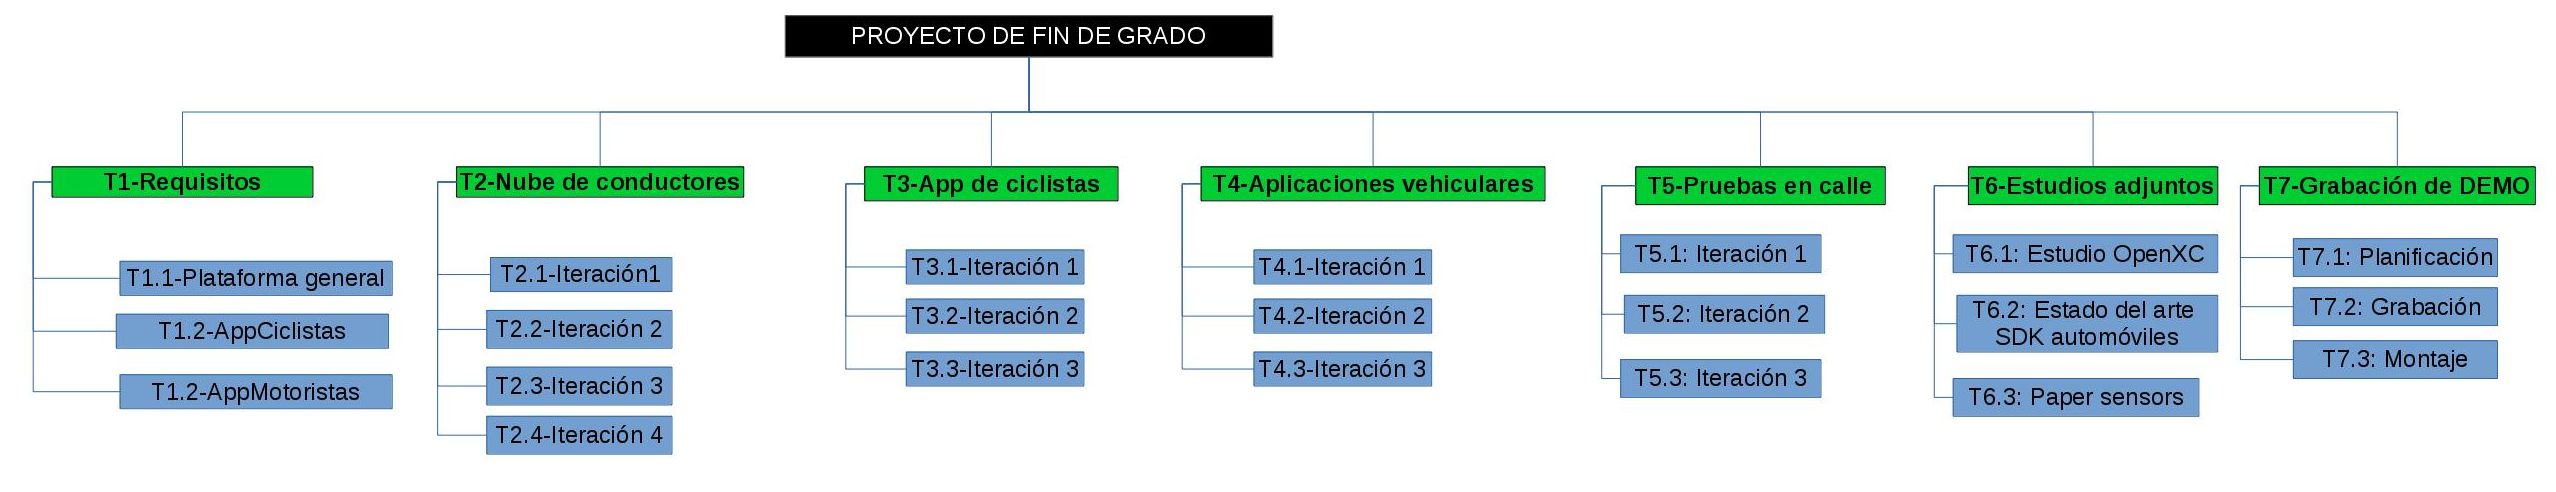
\includegraphics[scale=0.25]{EDT}
		}
		\caption{Diagrama de desglose de trabajo}
		\label{fig:EDT}
	\end{center}
\end{figure}
